\documentclass[10pt,a4paper]{article}
\usepackage[top=1.2cm,bottom=1.2cm,left=1.5cm,right=1.5cm]{geometry}
\usepackage{graphicx}
\usepackage{booktabs}
\usepackage{amssymb}
\setlength{\parskip}{0.3em}
\setlength{\parindent}{0pt}
\setlength{\abovecaptionskip}{2pt}
\setlength{\belowcaptionskip}{0pt}

\title{\textbf{VMC/RBM Results Overview}\\[0.1em]
       \large 1D TFIM and Long-Range 1D TFIM}
\author{}
\date{\today}

\begin{document}
\maketitle
\vspace{-2.2em}

% ─────────────────────────────────────────────────────────────────
\section*{1D TFIM — Sampler Comparison (N\,=\,32, h\,=\,0.5, full RBM)}
\vspace{-0.3em}
% ─────────────────────────────────────────────────────────────────

\begin{figure}[htbp]
  \centering
  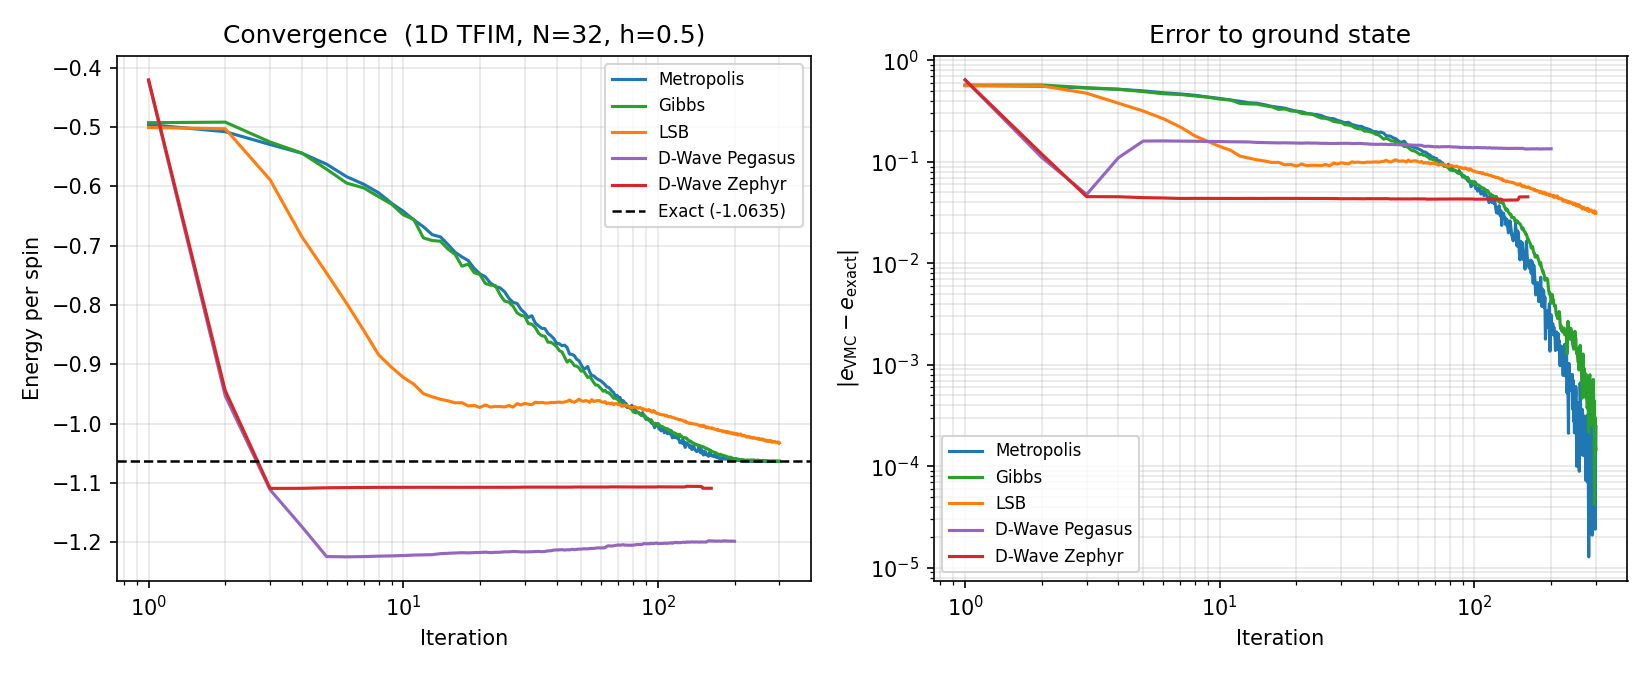
\includegraphics[width=0.92\linewidth]{convergence_N32_h0.5_all_samplers.png}
  \vspace{-0.4em}\\
  \small\textit{Energy per spin (left) and absolute error (right) for all sampler backends.
  Metropolis, Gibbs, and LSB converge to $\lesssim 10^{-4}$ per spin;
  D-Wave Pegasus and Zephyr plateau near $10^{-2}$.}
\end{figure}

\vspace{-1em}

% ─────────────────────────────────────────────────────────────────
\section*{1D TFIM — Error and Cost vs System Size}
\vspace{-0.3em}
% ─────────────────────────────────────────────────────────────────

\begin{figure}[htbp]
  \centering
  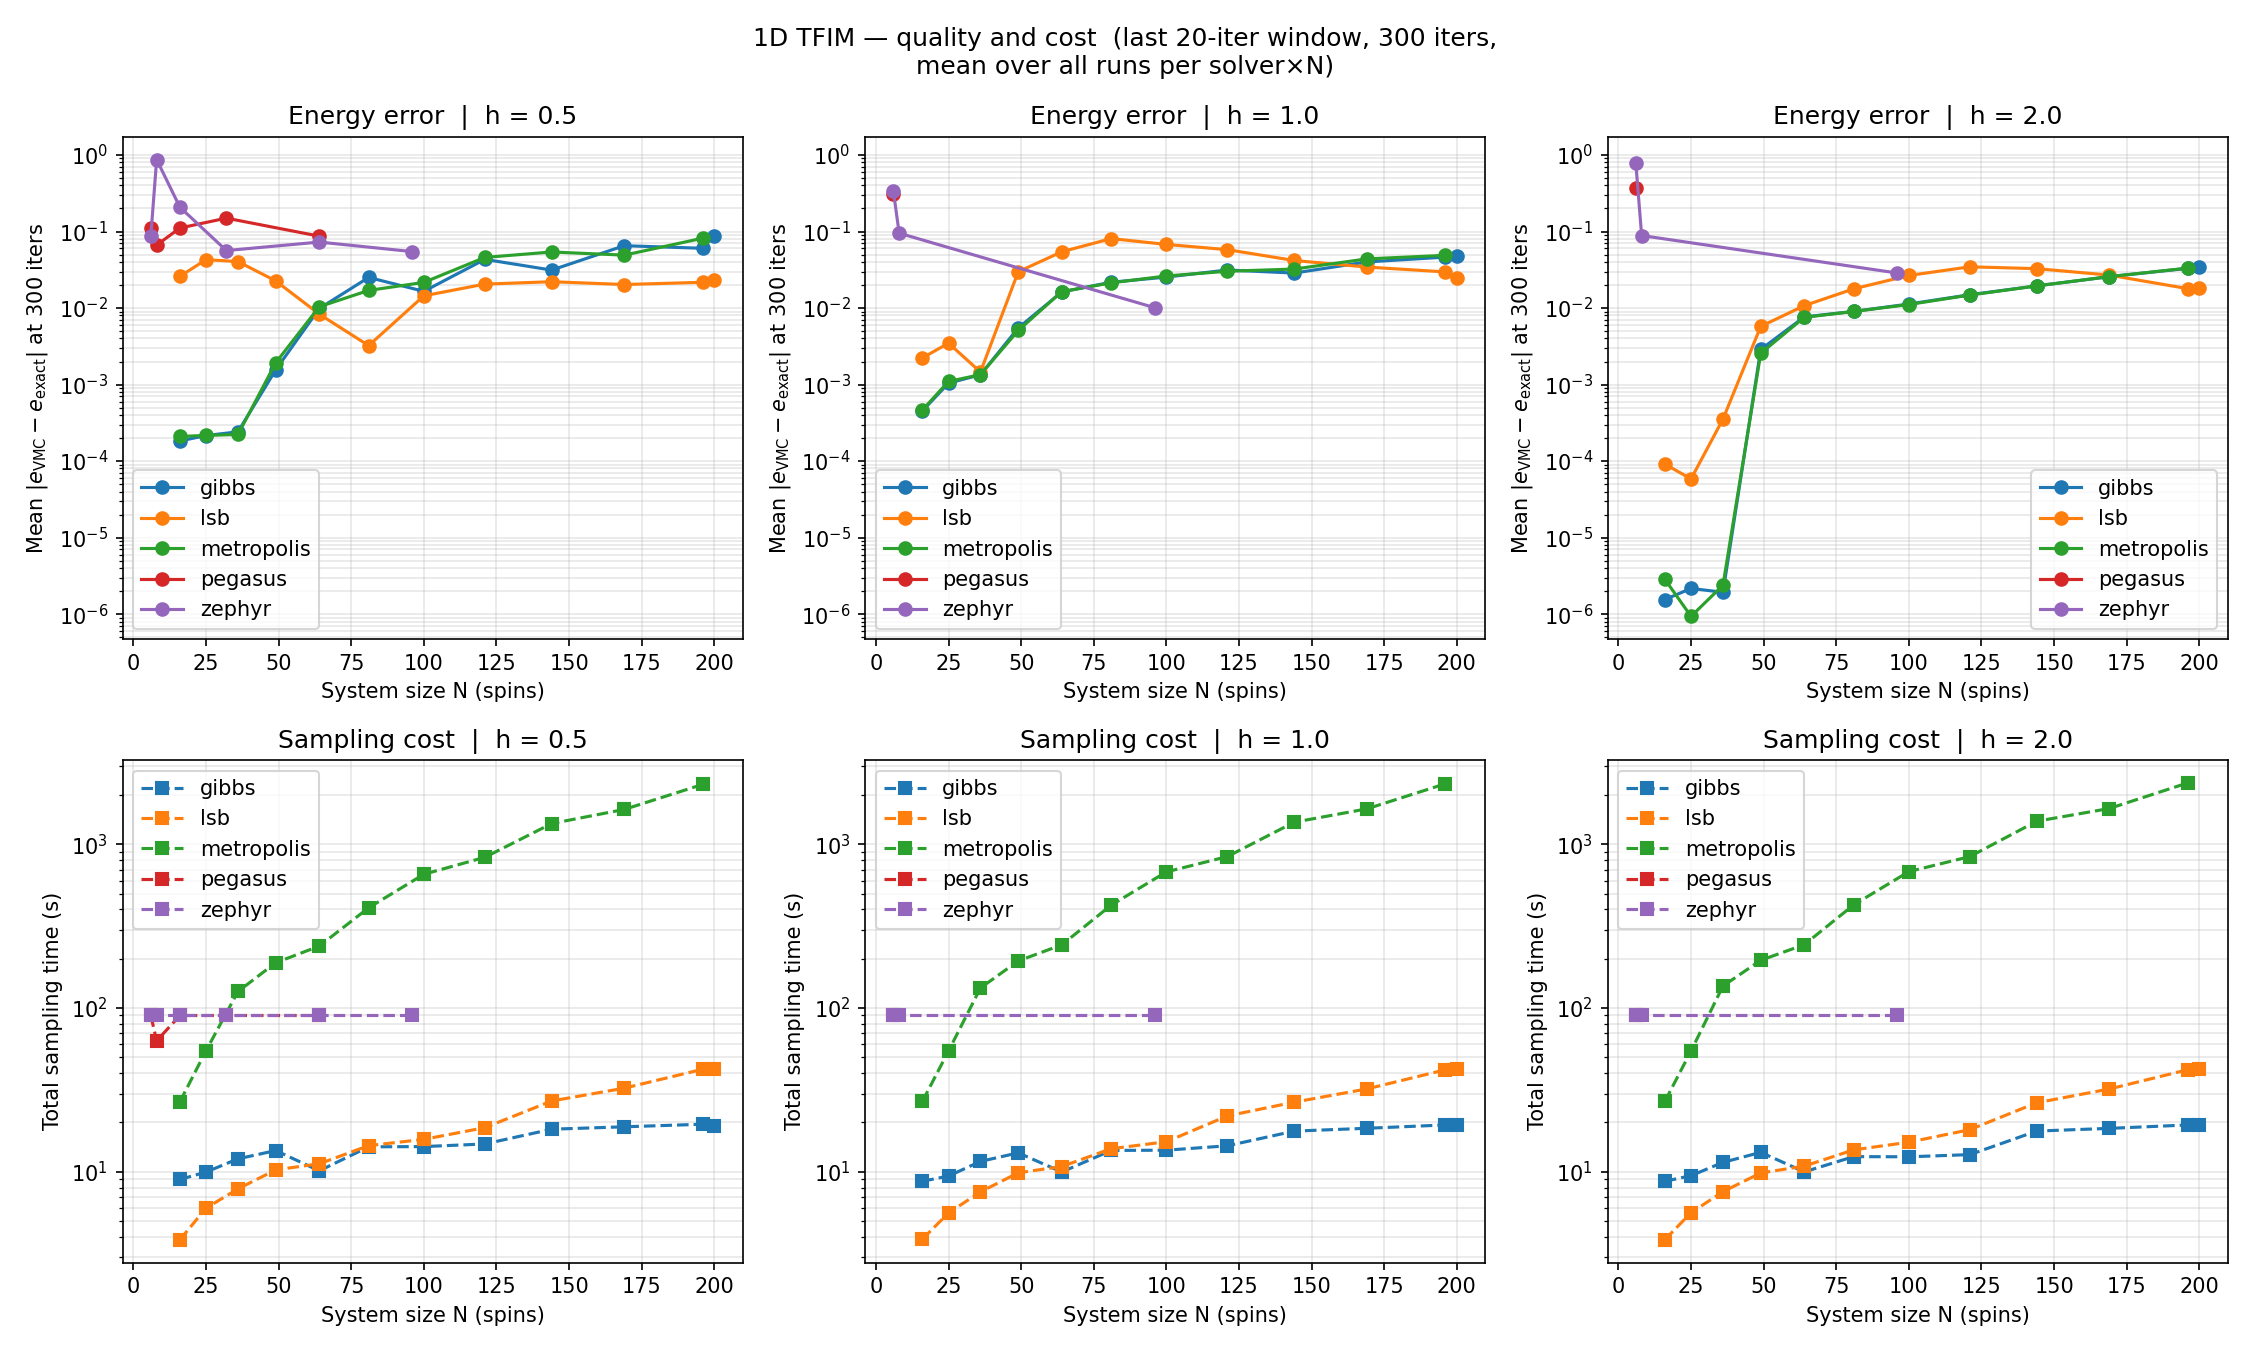
\includegraphics[width=0.96\linewidth]{../distance_vs_size.png}
  \vspace{-0.4em}\\
  \small\textit{Mean energy error per spin (top) and total sampling time (bottom)
  vs.\ $N$, for $h\in\{0.5,1.0,2.0\}$. Error measured in the last 20-iteration
  window of 300 iterations.}
\end{figure}

\newpage

% ─────────────────────────────────────────────────────────────────
\section*{Long-Range 1D TFIM — Error and Cost vs System Size}
\vspace{-0.3em}
% ─────────────────────────────────────────────────────────────────

$H = -J\sum_{i<j}\sigma^z_i\sigma^z_j/d(i,j)^\alpha - h\sum_i\sigma^x_i$,\quad
$d(i,j)=\min(|i-j|,N-|i-j|)$.\quad
$N\in\{16,25,36\}$; reference energy per spin from $N=16$ ED for $N>16$.

\begin{figure}[htbp]
  \centering
  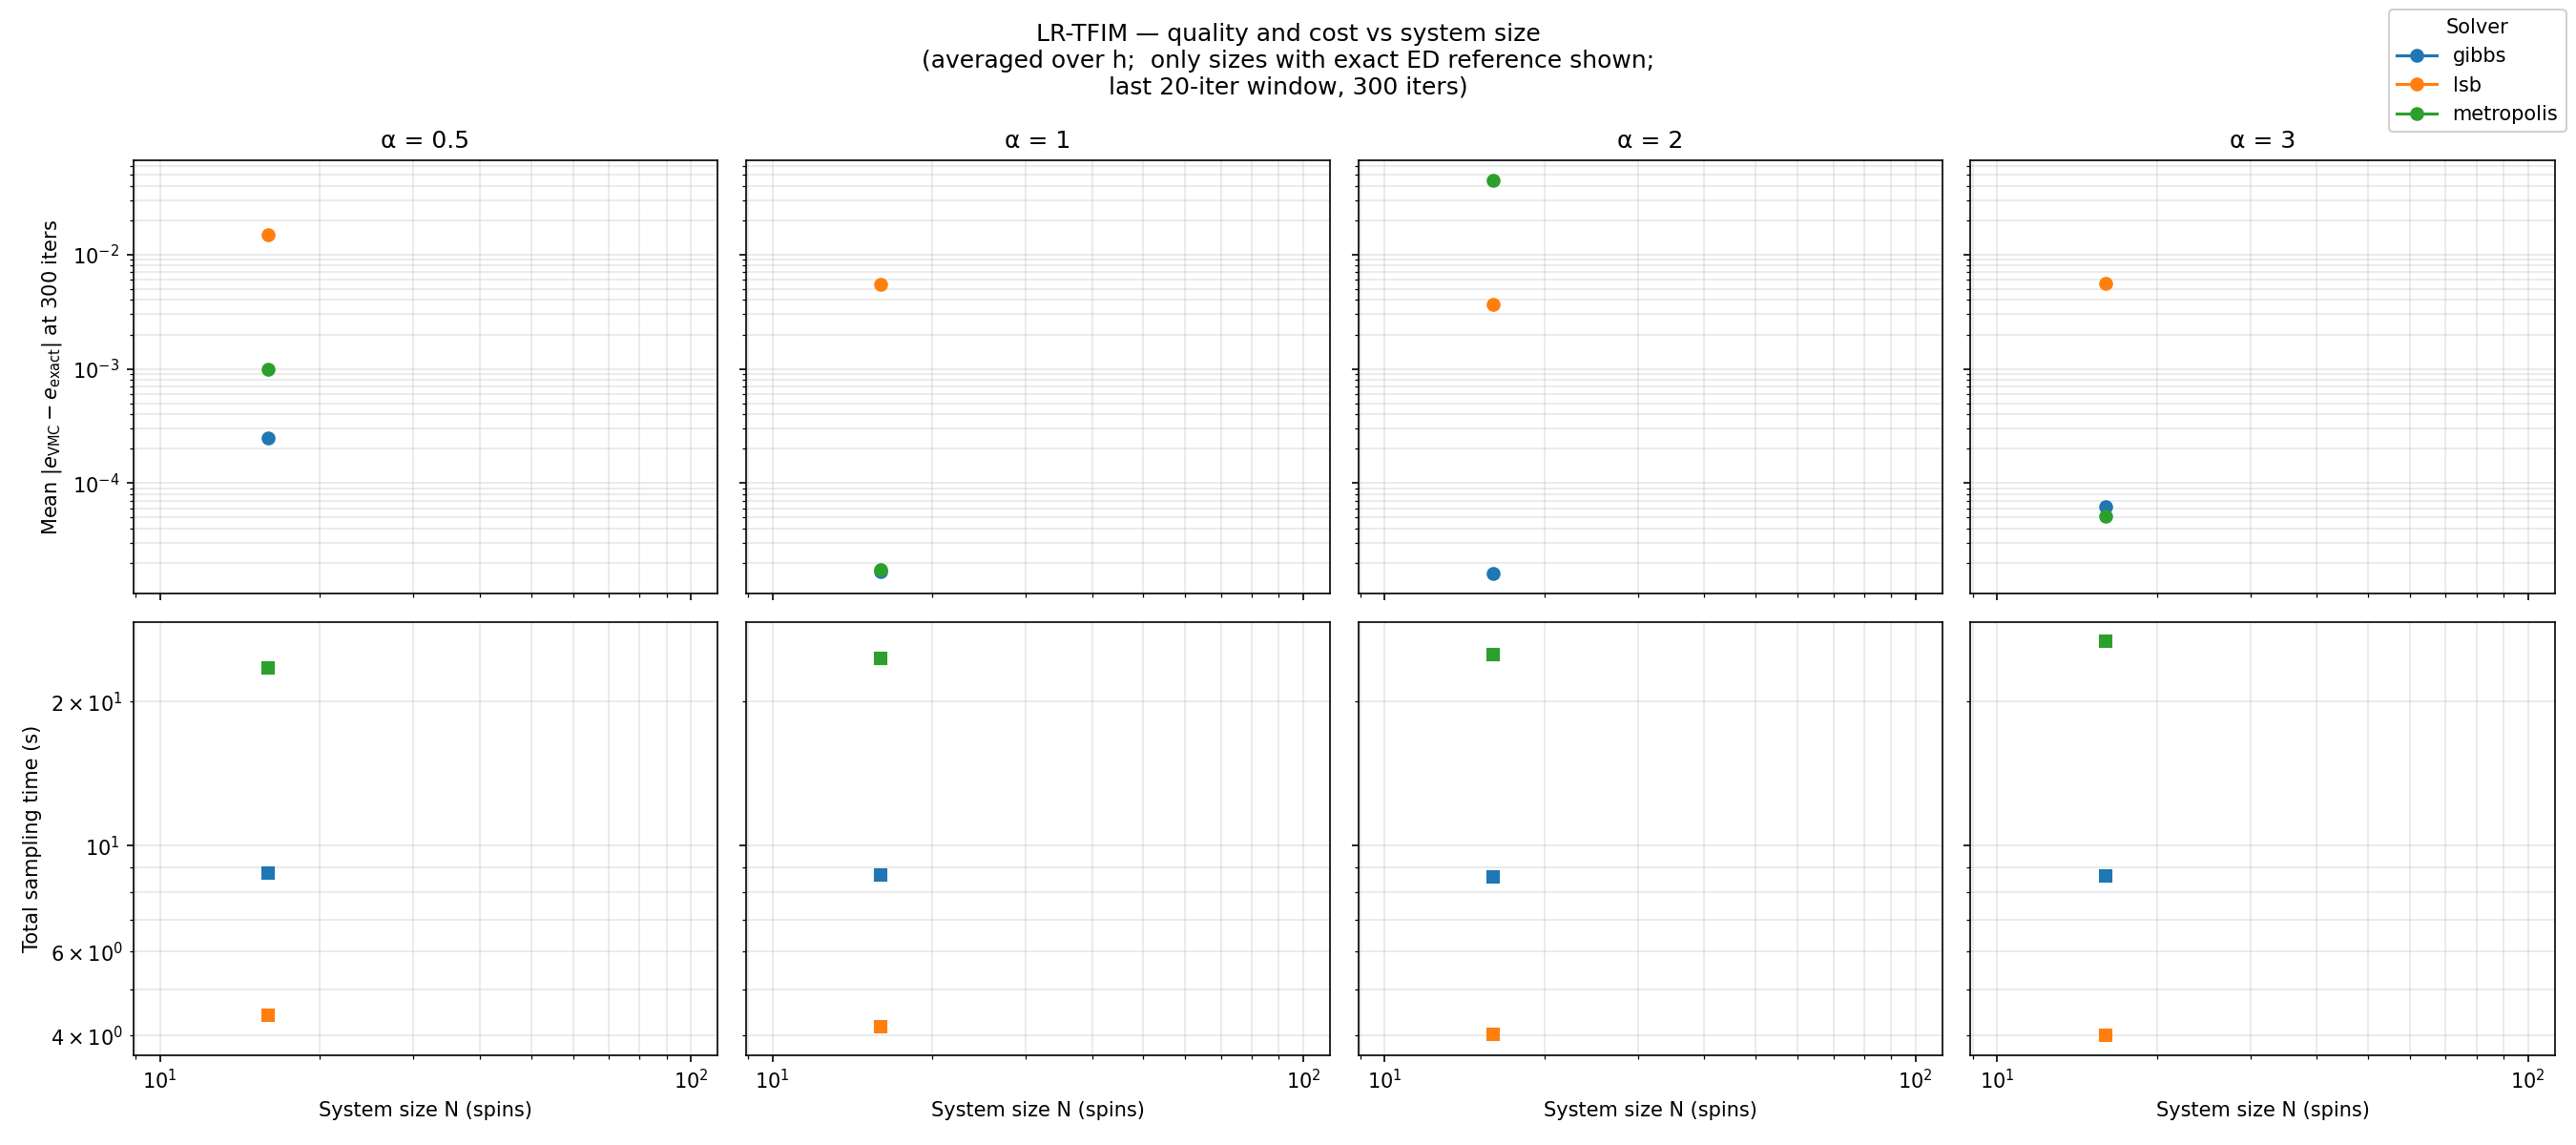
\includegraphics[width=0.96\linewidth]{../lr_tfim_distance_vs_size.png}
  \vspace{-0.4em}\\
  \small\textit{Same metrics as above, averaged over $h\in\{0.5,1.0,2.0,3.044\}$,
  one column per $\alpha$. Only $N=16$ shown: exact ED reference only available there;
  larger $N$ omitted because the per-spin ground state energy shifts with $N$
  (finite-size effect), making the N=16 reference an invalid baseline.}
\end{figure}

\vspace{-0.8em}

% ─────────────────────────────────────────────────────────────────
\section*{LR-TFIM vs.\ 1D TFIM — Direct Comparison at N\,=\,16}
\vspace{-0.3em}
% ─────────────────────────────────────────────────────────────────

\begin{figure}[htbp]
  \centering
  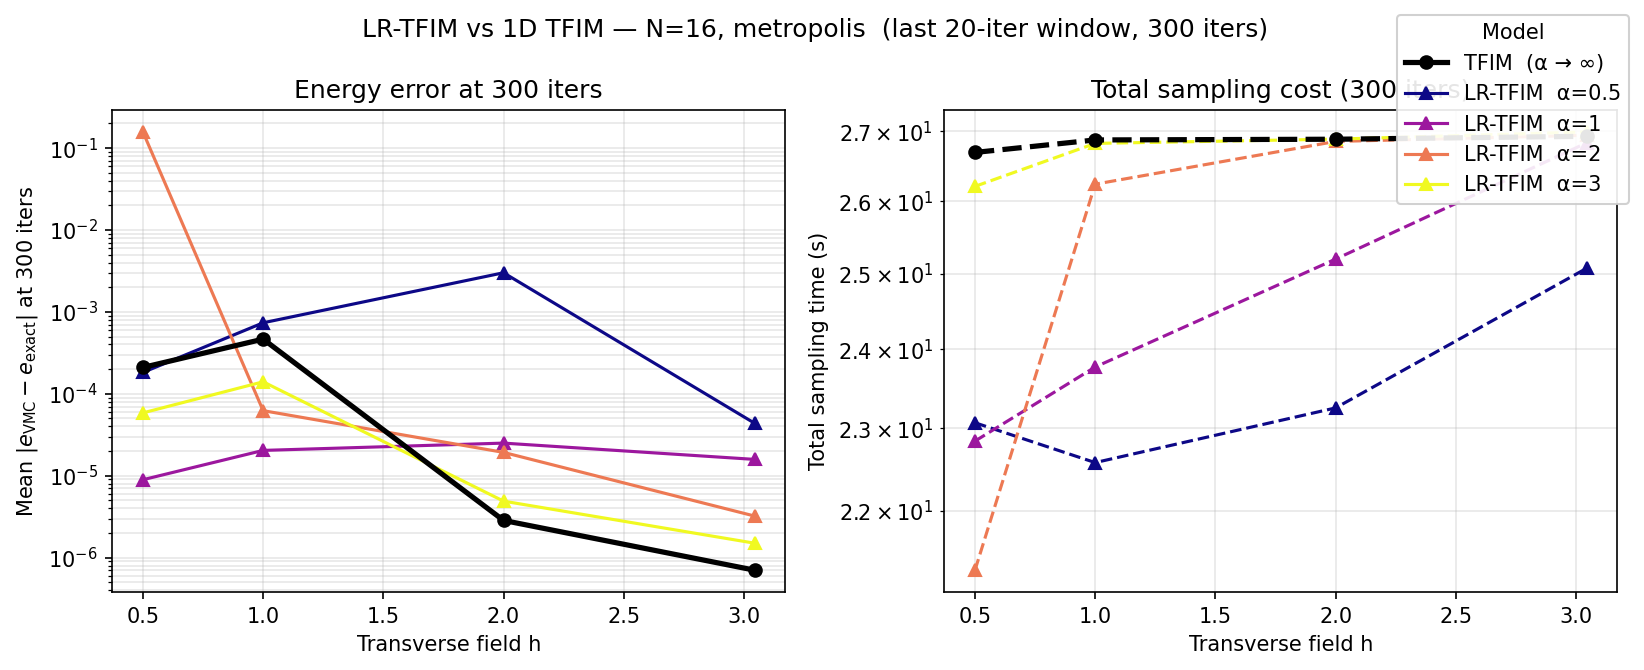
\includegraphics[width=0.92\linewidth]{../lr_vs_tfim_comparison.png}
  \vspace{-0.4em}\\
  \small\textit{Energy error (left) and total sampling time (right) vs.\ $h$,
  Metropolis sampler, last 20-iter window of 300 iterations.
  Black: nearest-neighbour TFIM ($\alpha\to\infty$).
  Coloured lines: LR-TFIM for $\alpha\in\{0.5,1,2,3\}$.}
\end{figure}

\end{document}
